\documentclass[a4paper,11pt]{article}
\usepackage{graphicx,listings,a4wide}
%\usepackage[firstpage]{draftwatermark}
%\SetWatermarkLightness{0.5}
%\SetWatermarkScale{4}
\setcounter{tocdepth}{2}

\newcommand{\question}[2]{\medskip\par\noindent\textbf{#1}\\\hangindent=0.5cm#2}

\title{Report on OGO 2.2 \\ Software specification\\ Testcases for group 3}
\author{
        Tim van Dalen\\ Tony Nan \and Ferry Timmers\\ Lasse Blaauwbroek\\ Femke Jansen \and Jeroen Peters\\ Sander Breukink \and OGO 2.2 group 6 \\
                Department of Computer Science\\
        Technical University Eindhoven\\
}
\date{\today}

\begin{document}

\maketitle

\begin{abstract}
This document contains several non-trivial test cases based upon the formal specification of group 3. In particular, we provide test cases for those scenarios that are not yet captured correctly in the formal specification. For each test case, we first provide a short description of the purpose of the test; then, we formally describe the input and output. In the testcases for the Z-specification, we describe the input and output in terms of the variables and types of the associated Z-schema.
\end{abstract}

    \section{Testcases for Z-specification}

\subsection{0 Pieces}
    Description: This test case is used to check the behavior of the system when an invalid number of pieces is entered. \\
    Scheme: Init.\\
    Input: $n?$ = 0.\\
    Output: An error message indicating that each player has to begin with at least one piece.

\subsection{Fox eats dolphin in water}
    Description: In this test case, a fox is two tiles away from the land and a dolphin is on a water tile between the fox and the land. In this scenario, the fox moves towards the land and ends up on the tile that is occupied by the dolphin. This scenario is a composition of RequestMove and DoKill. \\
    Scheme 1: RequestMove.\\
    Input 1: $x?$ and $y?$ are the destination coordinates of a water tile. $p?$ is a fox.\\
    Scheme 2: DoKill.\\
    Input 2: $x?$ and $y?$ are the same coordinates as before and there is a dolphin on $(x?,y?)$.\\
    Output: $movedXkilled! = (true,true)$.\\

    \subsection{Fox eats dolphin at bridge}
    Description: This test case is used to check the scenario of a flooded bridge where a dolphin is residing. The dolphin swam to one end of the bridge while it was flooded, but then the tide lowered and the dolphin could not move anymore. A fox then uses the bridge and kills the dolphin. This scenario is a composition of RequestMove and Tide.\\
    Scheme 1: RequestMove\\
    Input 1: $x?$ and $y?$ are the coordinates of one end of a bridge. $p?$ is a dolphin.\\
    Output 1: $movedXkilled! = (true,false)$.\\
    Scheme 2: Tide.\\
    Output 2: $e$ is a value low enough for the tile to go from sea to land.\\
    Scheme 3: RequestMove.\\
    Input 3: $x?$ and $y?$ are the coordinates of the other end of the bridge. $p?$ is a fox.\\
    Output 3: $movedXkilled! = (true,true)$.\\

    \subsection{Fox wants to go into the water}
    Description: a fox goes in to the water on purpose.\\
    Scheme: ReqeustMove.\\
    Input: $x?$ and $y?$ are the coordinates of the water tile the fox goes to, $p?$ is the fox itself.\\
    Output: If the tile was occupied by a dolphin the output becomes $movedXkilled! = (true,true)$, in all other cases the output becomes $movedXkilled! = (true,false)$.

    \subsection{Fox doesn't drown}
    Description: a fox is deep in the water and can't move anymore, but he stays alive. This scenario is a composition of RequestMove and Tide.\\
    Scheme 1: RequestMove.\\
    Input 1: $x?$ and $y?$ are the coordinates of a tile in the water. $p?$ is a fox.\\
    Output 1: $movedXkilled! = (true,false)$.\\
    Scheme 2: Tide.\\
    Output 2: $e$ is a value high enough to ensure that the fox is more than 2 tiles away from land.\\
    Scheme 3: RequestMove.\\
    Input 3: $x?$ and $y?$ are coordinates the fox wants to go to. $p?$ is the same fox.\\
    Output 3: $movedXkilled! = (false,false)$.\\


    Note: because we want to keep it a fair game, all testcases for foxes are also valid for the dolphin in the other way around.\\

	\section{Testcase for statechart}
	This MSC describes an execution of the statechart.

	Description: piece movement.

	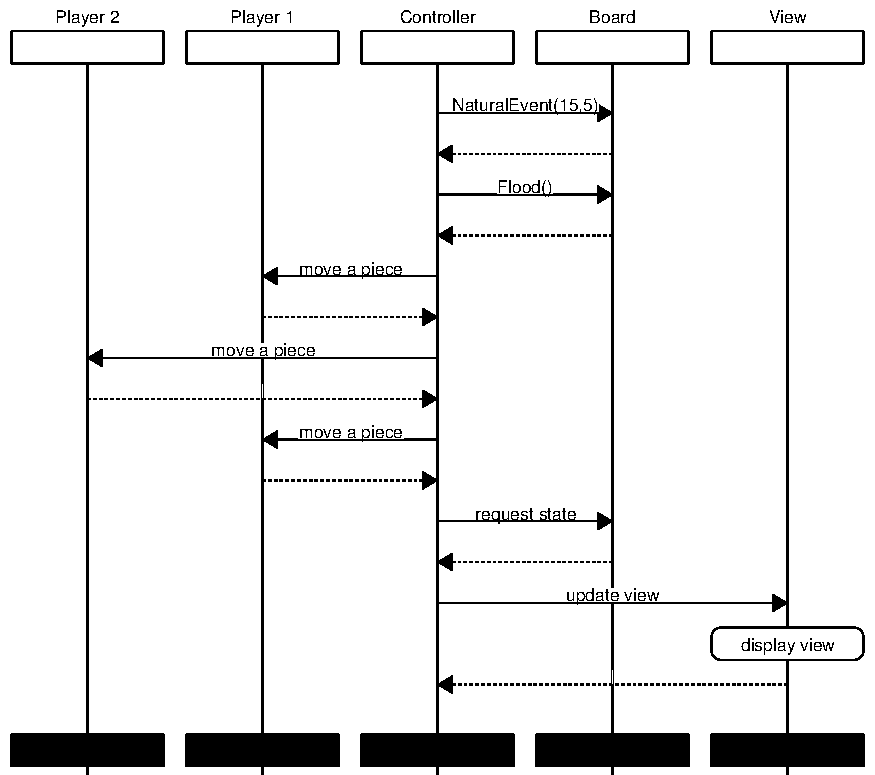
\includegraphics[width=\linewidth]{test_statechart}
\end{document} 
